\chapter{Homework 6}
\begin{minipage}{.70\textwidth}
\centering
\includegraphics[width=0.9\linewidth]{imgHW6/HW6}
\end{minipage}
\begin{minipage}{.70\textwidth}
\begin{tabular}{lcrl}
        DATA:\\
        l &	$=$	 & $50$	& $mm$\\
		g &	$=$ 	 & $2$		& $mm$\\
		t &	$=$	 & $1,5$ 	& $mm$\\
		wp &	$=$	 & $25$  	& $mm$\\
		Rp &	$=$ 	 & $4$		& $mm$\\
		Rd &	$=$	 & $3$ 		& $mm$\\
		$\delta$	 & $=$ 		& $4t$\\
		F 	&$=$ 	 & $100$ 	& $kN$\\
		Blank: &&S355JR &steel\\
		E 	&$=$	&$205$ 	& $GPa$\\
		$\sigma_{y}$ & $=$	&	$355$ & $MPa$\\
		Ep	 &$=$ & $4$ & $GPa$\\
\end{tabular}
\end{minipage}\\\\
The figure schematically illustrates the deep drawing of a metal sheet (blank). During the forming process, the blank is pressed against the die applying a preload $F$, then the punch is gradually displaced by $\delta$ in order to push the blank inside the die cavity. The stiffness of punch, die and blank holder is assumed to be much higher than that of the blank. The friction cofficient is $0,1$. Using axisymmetric plane elements, build a FE model able to simulate the forming process. In particular it is required to:
\begin{enumerate}
\item determine the distribution of the Von Mises equivalent stress at the end of the travel of the punch and the maximum axial force applied to the punch.
\item determine the punch stroke that maintains the maximum absolute hoop strain below $5 \%$.
\item determine the residual stress distribution on the top and the bottom surface of the blank after the punch removal.
\item determine the elastic springback, i.e. the difference in axial displacement prior to and after the punch removal of the points lying on the blank midplane.
\end{enumerate}
\section{Approach the problem}
This problem has created a model for the respective components: from the punch, through the use of keypoint and tracing lines to data provided by subsequently issue are made blankholder and die using the same procedure.\\
Then the blank is achieved the model as before, in the figure \ref{img:HW6-modelGeom}.\\
Summary characteristics of the blank holder, punch and die:
\begin{itemize}
\item The stiffness is assumed much higher than the blank, in fact it is not any material properties to the elements was attributed.
\item Displacement of punch: $\delta = 4*1,5 \, mm$;
\item Preload between blank holder - blank: $F = 100 \, kN$;
\end{itemize}
Instead, the blank has chosen to use:
\begin{itemize}
\item element type: \textsc{plane183};
\item using axisymmetric plane elements: \textsc{keyopt(3),1}
\end{itemize}
To realize the contact between the different components was used:
\begin{itemize}
\item the friction cofficient is $0.1$.
\item element type for rigid target body: \textsc{targe169};
\item element type for deformable contact body: \textsc{conta172};
\item optimization for deformable contact:
	\begin{itemize}
		\item Contact algorithm: \emph{Augmented Lagrangian}, \textsc{keyopt(2), 0}; 
		\item element level time incrementation control, \textsc{keyopt(7), 1}.\\ Automatic bisection of increment;
		\item To take into account the initial penetration or model initial interference, set \textsc{keyopt(9), 2}.\\ To ramp the initial penetration with the first load step (to model initial interference problems, for example);
		\item contact stiffness update for each iteration: \textsc{keyopt(10), 2}.
	\end{itemize}
\end{itemize}
\begin{figure}[!h]
\centering
\includegraphics[width=0.8\linewidth]{imgHW6/HW6-Geometry}
\caption{Complete geometry model}
\label{img:HW6-modelGeom}
\end{figure}
After these preliminary operations of the geometry creation is attributed to the stat blank mesh composed of elements such \textsc{plane183 }with optimization for axisymmetric. The elements have a length of $1 \, mm,$ at the same time for the entire height of $12$ divisions have been made. Finally you get the mapped mesh as show in figure \ref{img:HW6-Mesh}.
\begin{figure}[!h]
\centering
\includegraphics[width=0.8\linewidth]{imgHW6/HW6-Mesh}
\caption{Complete meshed model}
\label{img:HW6-Mesh}
\end{figure}\\\\
%%DISCUTERE DEGLI ELEMNTI DI CONTATTO
\noindent For molding simulation has chosen to use tree step, a first phase where the force is applied between the blank holder and the blank, as shown in the figure \ref{img:HW6-Solu_1}.
\begin{figure}[!h]
\centering
\includegraphics[width=0.8\linewidth]{imgHW6/HW6-Solu_1}
\caption{Pre gripping}
\label{img:HW6-Solu_1}
\end{figure}\noindent
The second phase is the descent of the die for a displacement of 6 mm, the last stage consists in stopping the die and in its ascent. The application of the load function is shown in the following chart \ref{img:HW6-Displacement}.
\begin{figure}[!h]
\centering
    \resizebox{.8\linewidth}{!}{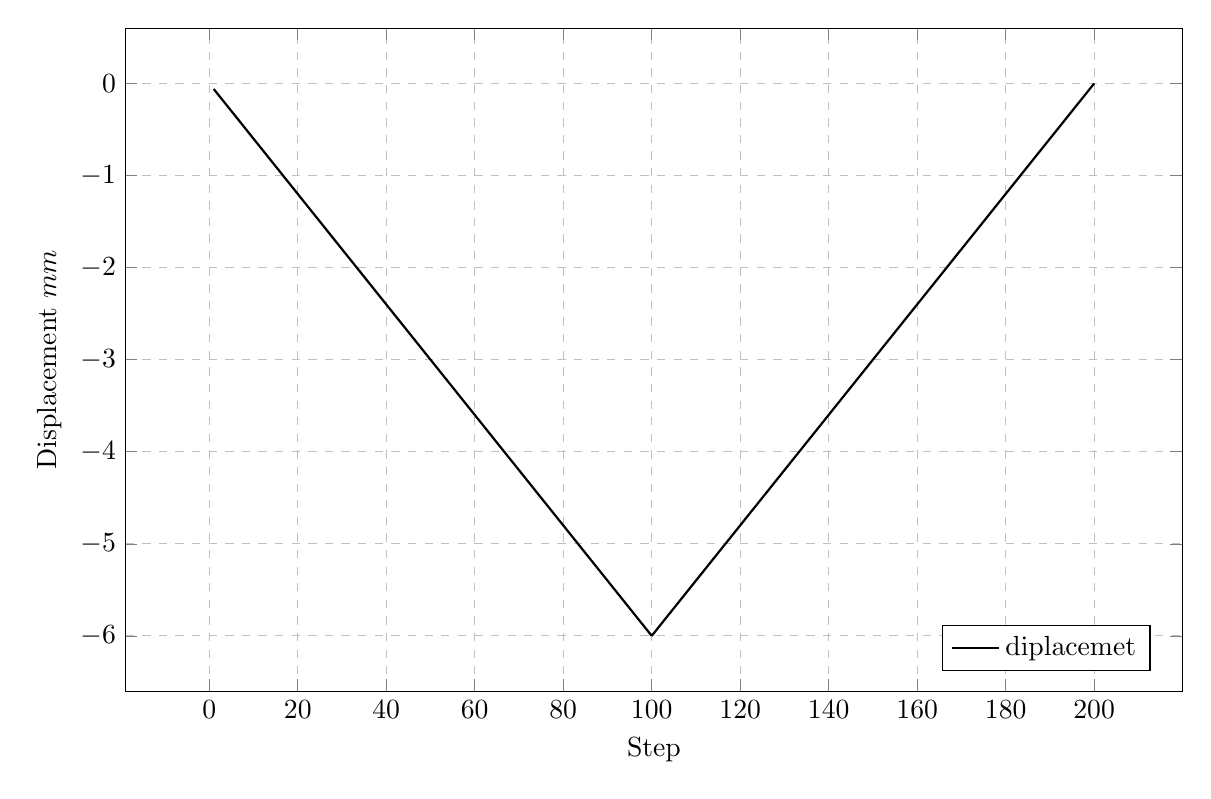
\begin{tikzpicture}
\pgfplotsset{major grid style={dashed},}
\begin{axis}[
						legend pos=south east,
						width=15cm,
						height=10cm,
						grid=major,
						ylabel=Displacement $mm$,
						xlabel=Step]
\addplot [thick, black, domain=1:100] {(-6/100)*x};
\addplot [thick, black, domain=100:200] {(6/100)*x-12};
\addlegendentry{diplacemet}
\end{axis}
\end{tikzpicture}}
    \caption{Load step die}
    \label{img:HW6-Displacement}
\end{figure}
It has opted for a high number of steps to avoid convergence problems during the solution phase, as in the first trials advised the program to increase the number of steps in the phase of application of the force as it was not able to find the solution after several iterations.
\section{Result and Conclusion}
%In the tuning options of the type \textsc{conta172} elements, you set the default method \emph{Augmented Lagrangian} as robust and present less sensitive to the magnitude of the contact stiffness.\\
The Von Mises equivalent stress at the end of the travel of the punch
and the maximum axial force applied to the punch, as show in figure \ref{img:HW6-Solu_101}.\\
\begin{figure}[!h]
\centering
\includegraphics[width=0.8\linewidth]{imgHW6/HW6-Solu_101}
\caption{Equivalent stress Von Mises}
\label{img:HW6-Solu_101}
\end{figure}\noindent
Max axial force applied to the punch is eqaul to $F = -58729,04097 \, N$.
\begin{figure}[!h]
\centering
    \resizebox{.8\linewidth}{!}{\begin{tikzpicture}
\pgfplotsset{cycle list={blue\\}, major grid style={dashed},}
\begin{axis}[
						legend pos=south east,
						width=15cm,
						height=10cm,
 						xmin=0, xmax=200,
        				ymin=-60000, ymax=1000,
        				grid=major,
        				ylabel=Force $N$,
        				xlabel=Step]
\addplot [thick, blue] table[smooth, mark=none, y=force, x=n]{HW6ForcePunch.txt};
\addlegendentry{Punch's force}
\end{axis}
\end{tikzpicture}}
    \caption{Force}
    \label{img:HW6-Force}
\end{figure}\\
%PARLARE HOOPSTRAIN
The punch stroke that maintains the maximum absolute, where is equal to $\sigma_{h} = 0,09445 \, MPa$, hence hoop stress close to the $5\,\%$ is equal $\sigma_{h5\%} = 0,0047 \, MPa$, hence the value of hoop strain is equal to $0,57169 \, mm$ as show in figure \ref{img:HW6-Hoopstrain}.
\begin{figure}[!h]
\centering
    \resizebox{.8\linewidth}{!}{\begin{tikzpicture}
\pgfplotsset{cycle list={orange\\pink\\purple\\red\\violet}, major grid style={dashed},}
\begin{axis}[
						width=15cm,
						height=10cm,
 						xmin=0, xmax=200,
        				grid= major,
        				xlabel=Step,
        				ylabel= Hoop strain $MPa$]
\addplot [thick, smooth, mark=none, Emerald] table [y={pHS}, x={n}]{HW6HoopStrain.txt};
\addplot [thick, smooth, mark=none, Emerald] table [y={nHS}, x={n}]{HW6HoopStrain.txt};
\draw [dash dot, red](axis cs:0,-0.0047) -- (axis cs:200,-0.0047) node [midway, above ] {
\textsc{\scriptsize \color{red}$5\,\%$}};
\draw [dash dot, red](axis cs:9.608941617,0) -- (axis cs:9.608941617,-0.0047);
\addlegendentry{Hoop strain}
\end{axis}
\end{tikzpicture}}
    \caption{Hoop strain below $5\, \%$}
    \label{img:HW6-Hoopstrain}
\end{figure}\\
When a metal forming tool is planned and designed to deform a work piece, the shape imparted by the tool will be a combination of elastic and plastic deformation, the release of the elastic deformation is the spring back often observed at the end of a metal forming process. The spring back has to be compensated to achieve an accurate result.\\The springback effect is visible in the follow graph \ref{img:HW6-Springback}.
\begin{figure}[!h]
\centering
    \resizebox{.8\linewidth}{!}{\begin{tikzpicture}
\pgfplotsset{cycle list={cyan\\magenta\\orange\\pink\\purple\\red\\teal\\violet\\yellow\\}, major grid style ={dashed, gray},}
\begin{axis}[
						legend cell align={left},
						legend pos=south east,
						width=15cm,
						height=10cm,
 						xmin=0, xmax=25,
        				ymin=-7, ymax=1,
						grid=major,
						xlabel=Radius $mm$,
						ylabel=Displacement $mm$]
\addplot [thick, smooth, mark=none] table[y=displacement, x=n]{HW6Set101.txt};
\addlegendentry{before remove punch}
\addplot +[stack plots=y, thick] table[smooth, mark=none, y=displacement, x=n ]{HW6Set103.txt};
\addlegendentry{after remove punch}
\addplot +[stack plots=y, stack dir=minus, thick ] table[smooth, mark=none, y=displacement, x=n]{HW6Set101.txt};
\addlegendentry{springback}
\end{axis}
\end{tikzpicture}}
    \caption{Springback effect}
    \label{img:HW6-Springback}
\end{figure}\\\noindent
Finally shows the plotted data showing the residual stress distribution on top and bottom surface of the blank after the punch removal, as in figures \ref{img:HW6-Solu_103}, \ref{img:HW6-TOP_Seqv} and \ref{img:HW6-BOT_Seqv}. 
\begin{figure}[!h]
\centering
\includegraphics[width=0.8\linewidth]{imgHW6/HW6-Solu_103}
\caption{Equivalent stress Von Mises}
\label{img:HW6-Solu_103}
\end{figure}
\begin{figure}[!h]
\centering
\includegraphics[width=0.8\linewidth]{imgHW6/HW6-TOP_SEQV}
\caption{Equivalent stress Von Mises top surface}
\label{img:HW6-TOP_Seqv}
\end{figure}
\begin{figure}[!h]
\centering
\includegraphics[width=0.8\linewidth]{imgHW6/HW6-BOT_SEQV}
\caption{Equivalent stress Von Mises bottom surface}
\label{img:HW6-BOT_Seqv}
\end{figure}
\clearpage
\section{Command list}
\begin{multicols}{2}
\scriptsize
\lstinputlisting[language=APDL, style=apdl-modified]{CommandList-HW6imgMOD.txt}
\normalsize
\end{multicols}